\documentclass[aps,pre,preprint,unsortedaddress]{revtex4}
% \documentclass[aps,pre,twocolumn]{revtex4-1}
% \documentclass[aps,jcp,groupedaddress,twocolumn,unsortedaddress]{revtex4}

\usepackage{amsmath}
\usepackage{amssymb}
\usepackage[dvips]{graphicx}
\usepackage{color}
\usepackage{tabularx}
\usepackage{algorithm}
\usepackage{algorithmic}

\makeatletter
\makeatother

\newcommand{\recheck}[1]{{\color{red} #1}}
\newcommand{\redc}[1]{{\color{red} #1}}
\newcommand{\bluec}[1]{{\color{blue} #1}}
\renewcommand{\v}[1]{\textbf{\textit{#1}}}
\renewcommand{\d}[1]{\textsf{#1}}


\begin{document}

\title{The theoretical considerations on the grand-canonical molecules dynamics simulation}
\author{Han Wang}
\affiliation{Institute for Mathematics, Freie Universit\"at Berlin, Berlin, Germany}
\author{Christof Sch\"utte}
\affiliation{Institute for Mathematics, Freie Universit\"at Berlin, Berlin, Germany}
\author{Luigi Delle Site}
\affiliation{Institute for Mathematics, Freie Universit\"at Berlin, Berlin, Germany}
\author{Other contributors should be added}

\begin{abstract}
\end{abstract}

\maketitle

\section{Introduction}

Atomistic molecules dynamics (MD) simulations are proved to be very
useful in studying the microscopic structure and functionality of
macromolecules, e.g.~\cite{shaw2010atomic}. However, even with the
constantly growing super-computer power, it is still impossible to
directly study some large-scale phenominon or long-time dynamics with
atomistic resolution. A promising way to overcome this obstacle is by
coarse-graining~\cite{voth2009coarse, peter2008classical,
  peter2009multiscale}, which reduces number of degrees of freedom
(DOFs) within a functional group, and at the same time, catches the
main structural properties (e.g backbone conformation) that are of
special interest. In some simulations, for example
Ref.~\cite{lambeth2010communication}, the atomistic details is
critical on the hydrophobic surface, while the coarse-grained
resolution is enough for the solvent environment far away. This gives
rise to the idea of adaptive resolution scheme
(AdResS)~\cite{praprotnik2005adaptive, praprotnik2006adaptive}, which
allow molecules change the representation from atomistic to
coarse-grained and {vice versa} on the fly, see Fig.~\ref{fig:tmp1}..
The periodic simulation box is devided into three regions: one
explicit region where molecule are atomistic, one coarse-grained
region and a hybrid region bridging the two representations together.
The identity of a molecule depends on its position, and is denoted by
a weighting function $w(\v r)$: the atomistic identity is denoted by
$w=1$, while the coarse-grained is $w=0$.  The molecules in the hybrid
region have both identities at the same time, and gradually change
their identity when travelling from atomistic to coarse-grained (or
vise versa).  More strictly, the weighting function smoothly and
monotonically varies from 1 to 0 (or 0 to 1). This change of identity
is also treated by the fractional change of the phase space
dimension~\cite{praprotnik2007adaptive1, praprotnik2007fractional}.

The AdResS method was successfully applied to study the tetrahedral
model molecules~\cite{praprotnik2006adaptive}, the liquid
water~\cite{matysiak2008modeling}, the hydrogen bond networks at the
hydrophobic interfaces~\cite{lambeth2010communication}, bridging
atomicstic water with continuous fluid dynamics
simulation~\cite{delgado2009coupling}, and was implemented in the MD
simulation package ESPResSo~\cite{junghans2010reference,
  limbach2006espresso}. Recently, the AdResS method was improved to
provide uniform local chemical potential all over the system, so the
thermodynamic equilibrium between different representations is
ensured~\cite{poblete2010coupling}.  Moreover, the AdResS method is
shown to conduct a grand-canonical simulation of the atomicstic
region, providing a thermodynamic force that ensures the uniform local
grand potential all over the system, and with the coarse-grained
region serveing as a particle reservior~\cite{fritsch2011grand}.
Although only be of theoretical interest, it is also possible to
consider the grand-canonical argument in the opposite way: the
atomicstic region serves as the particle reservior for the
grand-canonical simulation of coarse-grained molecules.
Unlike Monte Carlo (MC) simulation that can easily perform
grand-canonical simulation~\cite{allen1990computer}, the non-trival
grand-canonical MD simulation is lacking for a long time. The AdResS
method fill this gap in a very efficient way: the explicit region
where the physical properties are investigated is of full atomistic
resolution, while the particle reservior where molecular details are
not important is of coarse-grained resolution.

Ref.~\cite{fritsch2011grand} demostrate the method by a thermodynamic
arguement and verify the grand-canonical simulation numerically.  The
aim of the present paper is to provide a strict theoretical basis for
the grand-canonical AdResS method by the statistical physics
arguments, and some necessary but not suffcient conditions.  The paper
is arranged as follow: in section~\ref{sec:theory}, the
grand-canonical AdResS simulation method is shortly introduced, and
then the method is discussed and analyzed in the strict statistical
physics way. The nesscessary conditions for grand-canonical AdResS
simulation is summarize in the end of this section. In
section~\ref{sec:rdf-corr}, a numerical method is developed to fulfill
all the proposed condition at the same time. The validation of the
method is proved by the AdResS simulation of liquid water.  This paper
is summrized and concluded in section~\ref{sec:conclusions}.




\section{Theory}\label{sec:theory}


\begin{figure}
  \centering
  % 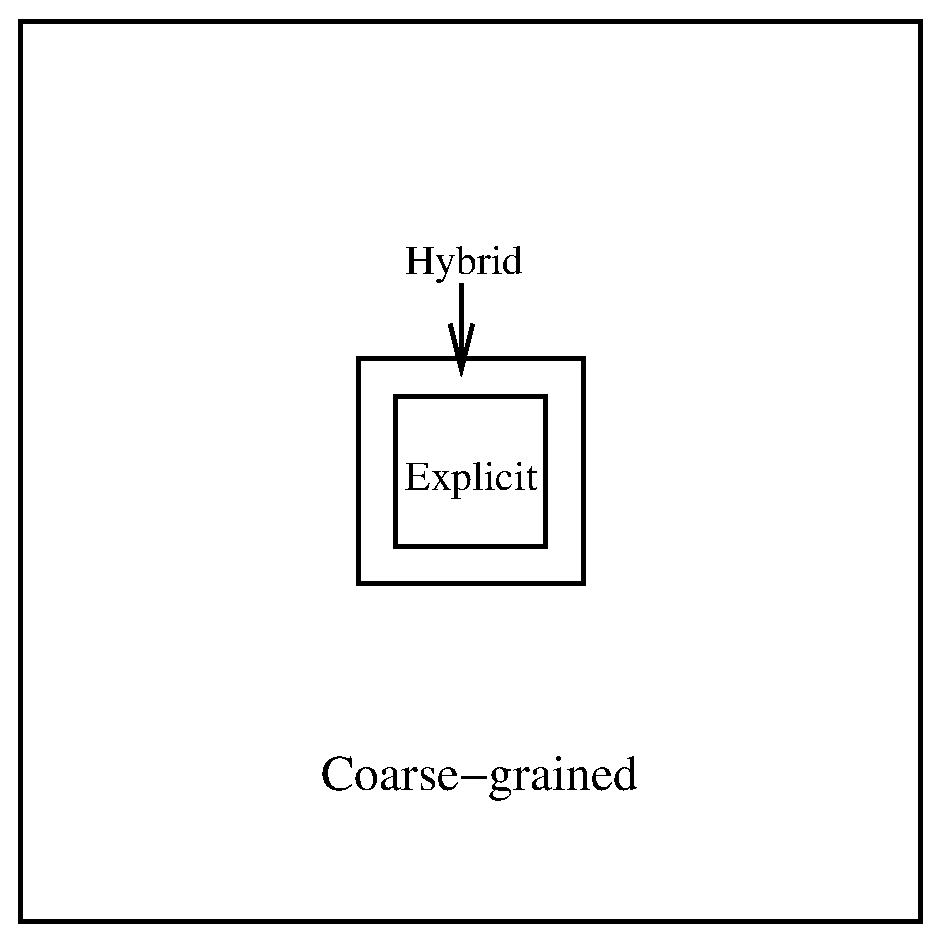
\includegraphics[width=.5\textwidth]{fig/system/system.eps}
  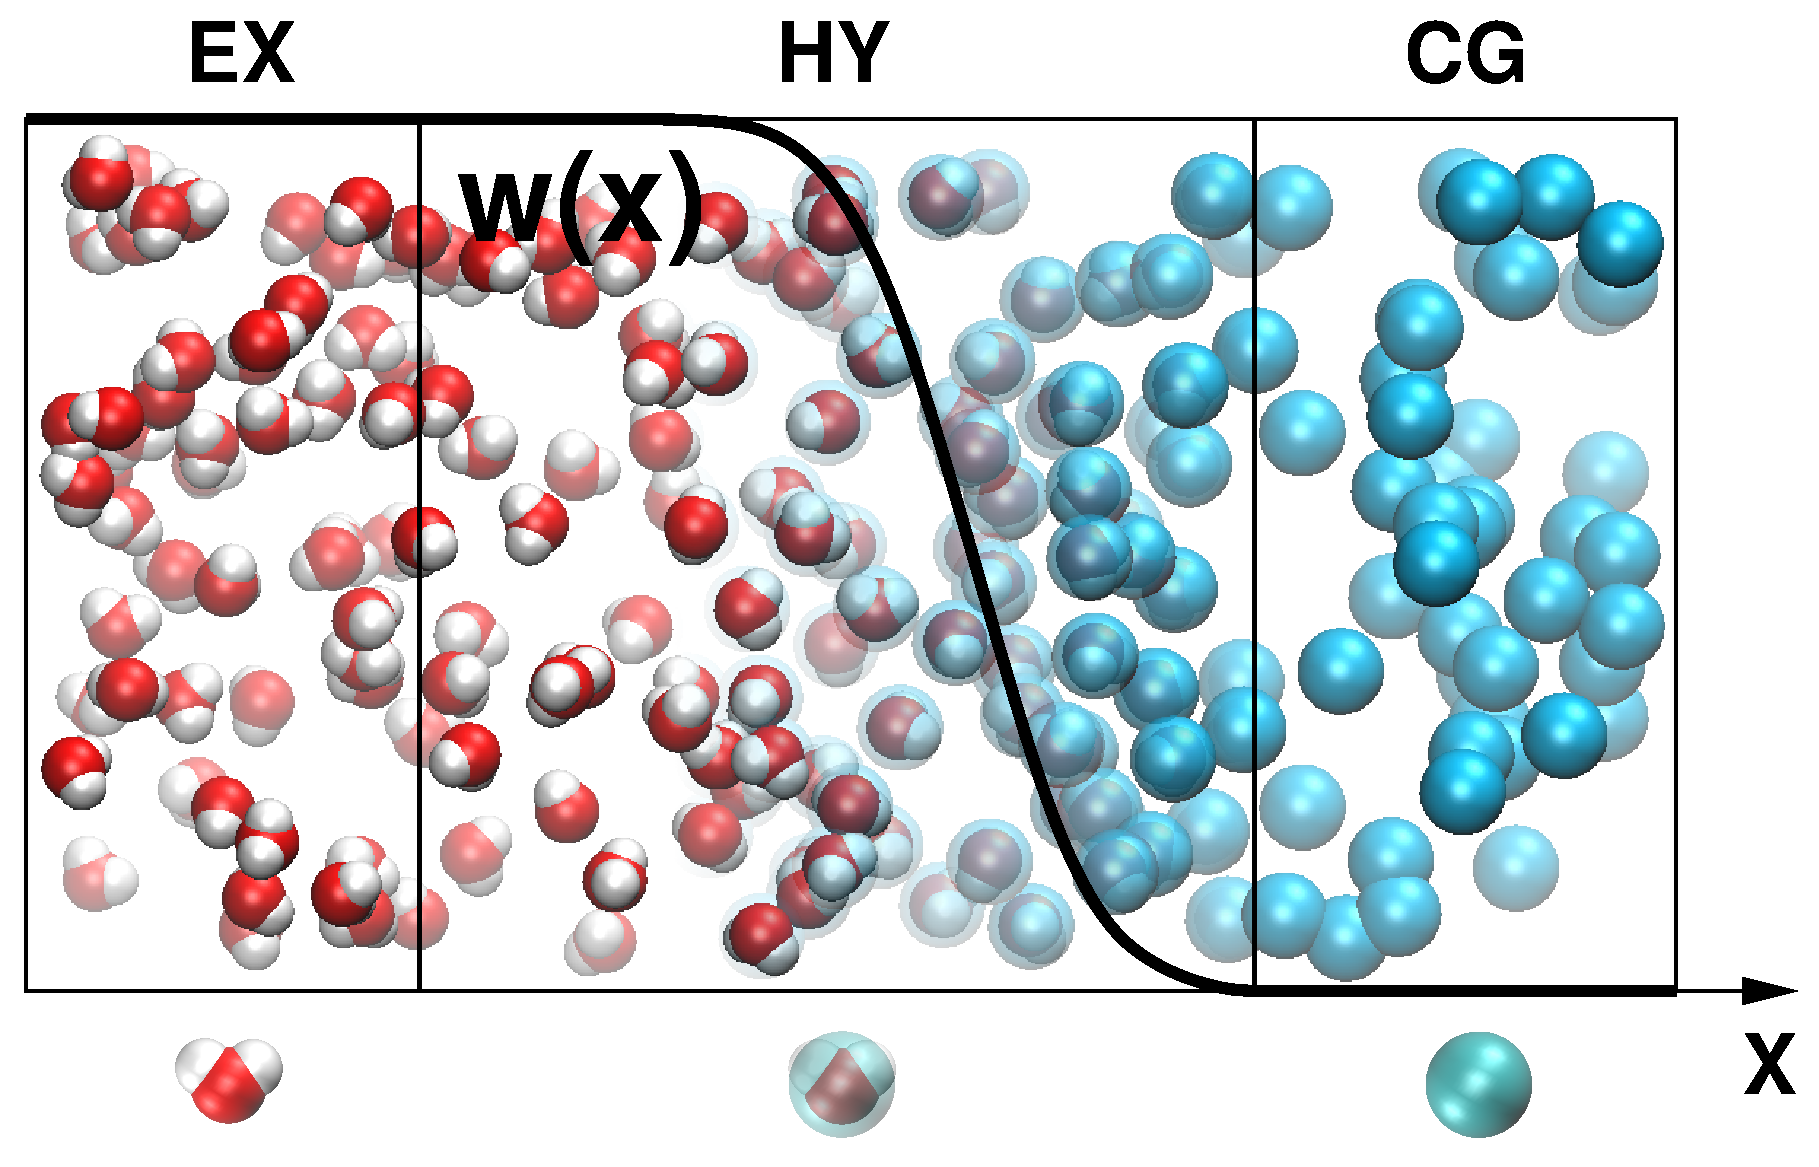
\includegraphics[width=.5\textwidth]{fig.3/system/system.eps}
  \caption{An AdResS system}
  \label{fig:tmp1}
\end{figure}


We want to prove the trajectory of the explicit region in AdResS
simulation is an implementation of the $\mu$VT distribution. We take a
sequence of snapshots of the system along the trajectory.  For sure,
the number of molecules in the explicit region varies. We group the
snapshots by the number of molecules in the explicit region.  The
strategy of our prove is firstly to shown the position and
velocity distribution in each group, where the number of molecules
in the explicit region is fixed, is subject to the Boltzmann
distribution. Secondly, we show the number of snapshots in each group
is subject to the exponential distribution. Then the combination of
these two distributions ends up with the grand-canonical distribution.

Notice, the prove always compare the explicit region to an sub-system
of a big all-atom canonical system. If the explicit region is embedded
into the whole AdResS system in the same manner as the sub-system
embedded in to the big all-atom canonical system, then the AdResS will
give the correct grand-canonical distribution.


Consider the dynamics of a system that is subject to the Langevin equation:
\begin{align}
  \d d\v r_i &= \v v_i\d dt\\
  m_i\d d\v v_i &= [-m_i\xi_i\v v_i + \v F_i]\,\d dt + \sqrt{2\sigma_i}\,\d d\v W_t
\end{align}
where $\d d\v W_t$ is the standard Wiener process.  If the system has a
potential, namely $\v F_i = -\nabla_{\v r_i}U$, then it can be proved that the
Langevin dynamics generates the canonical ensemble:
\begin{align}
  p(\v r_1, \cdots, \v r_N, \v v_1, \cdots, \v v_N)
  = \exp\big[
  -\beta \mathcal H(\v r_1, \cdots, \v r_N, \v v_1, \cdots, \v v_N)
  \big]
  % \bigg[
  % \sum_i^N\frac12 m_i\v v_i^2 + U(\v r_1, \cdots, \v r_N)
  % \bigg]
\end{align}
where $\mathcal H$ is the Hamiltonian of the system:
\begin{align}
  \mathcal H(\v r_1, \cdots, \v r_N, \v v_1, \cdots, \v v_N)
  =
  \sum_{i=1}^N\frac12 m_i\v v_i^2 + U(\v r_1, \cdots, \v r_N)  
\end{align}

For the AdResS simulation, let us first consider there are $N_1$
molecules in the explicit region, $N_2 - N_1$ molecules in the hybrid
region.  Without lost of generality, we assume molecules $1, \cdots,
N_1$ are in the explicit region, molecules $N_1 + 1, \cdots, N_2$ are
in the hybrid region and $N_2+1, \cdots, N$ are in the coarse-grained
region. The pair $\{\v r_i, \v v_i\}$ of the explicit representation
denotes the center-of-mass (COM) position and velocity of the $i$-th
molecule. For convenience, we only consider the COM coordinate of the
explicit molecule, all the prove can be easily extended to treat every
atom the the molecule.

We hereby consider the explicit region as a sub-system of the whole
system, which composes the explicit, hybrid and coarse-grained
regions. We want to prove that the explicit region can be viewed as a
$\mu$VT sub-system, which is embedded into a huge NVT environment.
For any molecule $i$ in the explicit region, the force exerting on
it is
\begin{align}
  \v F_i &= \sum_{j=1}^{N}\v F_{ij} 
  =
  \sum_{j=1}^{N_1}\v F_{ij} + \sum_{j=N_1+1}^{N_2}\v F_{ij} 
\end{align}
Here it is assumed that the width of the hybrid region is larger than
the cut-off of the pairwise interaction $\v F_{ij}$, so the molecule
in the explicit region is not interacting with the molecules in the
coarse-grained region, as this happens in all applications.
The AdResS force interpolation scheme reads:
\begin{align}\label{eqn:f-interp}
  \v F_{ij} = w_iw_j\v F^{\textrm{ex}}_{ij} + [1-w_iw_j]\v F^{\textrm{cg}}_{ij},
\end{align}
where $w_i = w(\v r_i)$ represents
the resolution of the molecule:
\begin{align}\label{eqn:w1}
  w(\v r) =
  \left\{
    \begin{array}{lcl}
      1 &\quad& \textrm{atomistic region}\\
      0<w<1  && \textrm{hybrid region}\\
      0 && \textrm{coarse-grained region}.
    \end{array}
  \right.
\end{align}
The original AdResS papers proposed the weighting function:
\begin{align}\label{eqn:old-w}
  w(\v r) =
  \left\{
    \begin{array}{lcl}
      1 &\quad& \chi < d_{\textrm{ex}}\\
      \cos^2\big[\frac{\pi}{2(d_{\textrm{hy}})} (\chi - d_{\textrm{ex}})\big] && d_{\textrm{ex}}  < \chi < d_{\textrm{ex}} + d_{\textrm{hy}} \\
      0 && d_{\textrm{ex}} + d_{\textrm{hy}}  < \chi.
    \end{array}
  \right.
\end{align}
In the present work, we propose the following weighting function:
\begin{align}\label{eqn:new-w}
  w(\v r) =
  \left\{
    \begin{array}{lcl}
      1 &\quad& \chi < d_{\textrm{ex}}\\
      1  && d_{\textrm{ex}} < \chi < d_{\textrm{ex}} + r_c\\
      \cos^2\big[\frac{\pi}{2(d_{\textrm{hy}} - r_c)} (\chi - d_{\textrm{ex}} - r_c)\big] && d_{\textrm{ex}} + r_c < \chi < d_{\textrm{ex}} + d_{\textrm{hy}} \\
      0 && d_{\textrm{ex}} + d_{\textrm{hy}}  < \chi.
    \end{array}
  \right.
\end{align}
Where $d_{\textrm{ex}}$ and $d_{\textrm{hy}}$ are the size of the
explicit and hybrid region, respectively. $r_c$ is the cut-off
radius. Here $d_{\textrm{hy}} \geq 2r_c$. $\chi$ is the distance to
the border of the explicit region.  The molecules in the hybrid region
is applied a thermodynamic force $\v F^{\textrm{th}}(\v x)$
\begin{align}
  \v F_i = \sum_j\v F_{ij} + \v F^{\textrm{th}}(\v x_i),
\end{align}
which is defined to ensure a uniform grand potential:
\begin{align}
  \bigg(
  p(\v x_0) +
  \frac{\rho}{M}\int_{\v x_0}^{\v x_1}\v F^{\textrm{th}}(\v s)\,\d d\v s
  \bigg) V
  =
  p(\v x_1) V
\end{align}
From thermodynamic point of view, the thermodynamic force will lead
to the same chemical potential for the explicit and coarse-grained regions.
% This definition of $w(\v r)$ is \emph{different from the convention}, which
% has a value of 1 for the atomistic region and 0 for the coarse-grained
% region.

By the definition of the force interpolation scheme
\eqref{eqn:f-interp} and \eqref{eqn:new-w}, the interaction between the
explicit molecules and hybrid molecules is
\begin{align}
  \v F_{ij} = \v F^{\textrm{ex}}_{ij}
\end{align}
and obviously in the explicit region
\begin{align}
  \v F_i =
  \sum_{j=1}^{N_1}\v F^{\textrm{ex}}_{ij} + \sum_{j=N_1+1}^{N_2}\v F^{\textrm{ex}}_{ij}, \quad 1\leq i \leq N_1
\end{align}
Therefore, if we fix the coordinates of the molecules in the hybrid
region, the Hamiltonian of the explicit region can be written as
\begin{align}
  \mathcal H^{\textrm{ex}}(\v x_1; \v x_2) =
  \sum_{j=1}^{N_1}\frac12 m_i\v v_i^2 + 
  \sum_{i,j=1}^{N_1}\frac12 U^{\textrm{ex}}(\v r_i - \v r_j) + 
  \sum_{i=1}^{N_1}\sum_{j=N_1+1}^{N_2} U^{\textrm{ex}}(\v r_i - \v r_j) 
\end{align}
We denote the phase space variables: $\v x_1 = (\v r_1, \cdots, \v
r_{N_1}, \v v_1, \cdots, \v v_{N_1})$,  $\v x_2 = (\v r_{N_1+1},
\cdots, \v r_{N_2}, \v v_{N_1+1}, \cdots, \v v_{N_2})$ and
$\v x_3 = (\v r_{N_2+1},
\cdots, \v r_{N_3}, \v v_{N_2+1}, \cdots, \v v_{N_3})$.
Here $\v x_1$ is the variable and $\v x_2$ is considered as environment, 
by the Langevin dynamics, we have the conditional probability distribution
\begin{align}
  p (\v x_1 \vert \v x_2)  =
  e^{-\beta \mathcal H^{\textrm{ex}}(\v x_1; \v x_2)}
\end{align}
The phase space distribution of the explicit region:
\begin{align}
  p(\v x_1) = \int p(\v x_1\vert\v x_2)\cdot p (\v x_2) \,\d d\v x_2
\end{align}
If the phase space distribution $p(\v x_2)$ is the same as the explicit
Boltzmann distribution, then the explicit region is
equivalently embedded in to a explicit molecular environment and can be
viewed as a sub-system of a very big explicit molecular
system.

The crucial question is if $p(\v x_2)$ is correct.  A necessary
condition is that both the density and the radial distribution
function (RDF) are correct in the hybrid region. By the thermodynamic
force correction, the density is correct. Now the RDF...  If the
coarse-grained potential is generated by fitting the explicit RDF,
\redc{then in the hybrid region, it seems the RDF should not deviate very
  far from the correct.}

\begin{figure}
  \centering
  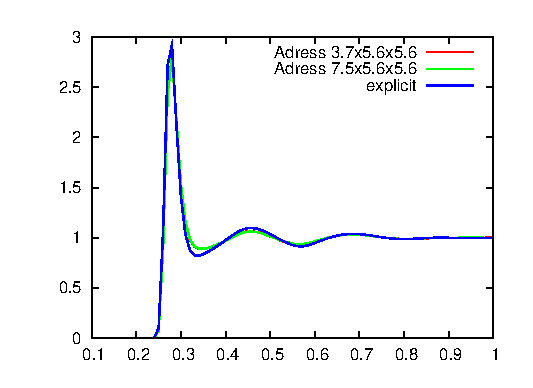
\includegraphics[]{fig/old.rdf/rdfs.eps}
  \caption{The RDF is independent with the size of the hybrid region.
    In the AdResS simulation, the whole region is defined hybrid. They
    are compared with the explicit water RDF.}
  \label{fig:tmp2}
\end{figure}

\bluec{
  What we want to do next is
  \begin{itemize}
  \item Theoretically show under what kind of condition the RDF is
    correct.
  \item We find the current AdResS scheme (with thermodynamic force
    applied) will not give perfect RDF in the hybrid region. However,
    the RDF profile is independent with the size of the hybrid region
    see Fig. \ref{fig:tmp2}. This fact gives rise to the idea of
    applying additional correction force in the hybrid region to fit
    the RDF, a possible form is
    \begin{align}
      \v F_{ij} = w_iw_j\v F^{\textrm{ex}}_{ij} + [1-w_iw_j]\v F^{\textrm{cg}}_{ij} +
      4 w_iw_j (1 - w_iw_j)\v F_{ij}^{\textrm{rdf}},
    \end{align}
    notice the thermodynamic force should also be added
    \begin{align}
      \v F_i = \sum_j\v F_{ij} + \v F^{\textrm{th}}(\v x_i),
    \end{align}
    The correction force $\v F_{ij}^{\textrm{rdf}}$ that is only
    applied in the hybrid region can be obtained by the
    coarse-graining method that fits the RDF, for example, the inverse
    Boltzmann interaction. 
  \end{itemize}
}
  

% \section{The distribution of $N$}
Fix the number in the three regions, both the explicit and the
coarse-grained regions are subject to the Boltzmann distribution. The
partition functions reads
\begin{align}\nonumber
  q(N,V,T)
  &= \frac1{N!}\int
  \d d\v x_1\d d\v x_3\,
  e^{-\beta
    [\mathcal H_1(\v x_1, N_1) + \mathcal H_3(\v x_3, N_3)]}\\\nonumber
  & = \frac{N_1!N_3!}{N!}
  \frac{1}{N_1!}\int\d d\v x_1 e^{-\beta\mathcal H_1(\v x_1, N_1)}
  \frac{1}{N_3!}\int\d d\v x_3 e^{-\beta\mathcal H_3(\v x_3, N_3)}\\
  & = \frac{N_1!N_3!}{N!}
  Q_1(N_1, V_1, T)
  Q_3(N_3, V_3, T) 
\end{align}
Considering the mutation of particles, the number of possibilities of
$N_1$ molecules being in the explicit region and $N_3$ molecules being
in the coarse-grained region is
\begin{align}
  \frac{N!}{N_1!N_3!}
\end{align}
Therefore, the partition function reads
\begin{align}\nonumber
  Q(N,V,T) &= \sum_{N_1}
  \frac{N!}{N_1!N_3!} \frac{N_1!N_3!}{N!}
  Q_1(N_1, V_1, T)\,
  Q_3(N_3, V_3, T) \\
  &= \sum_{N_1}
  Q_1(N_1, V_1, T)\,
  Q_3(N_3, V_3, T) 
\end{align}
The phase space distribution of the whole system is
\begin{align}
  p(\v x, N) = \frac{1}{Q(N,V,T) N!} e^{-\beta\mathcal H(\v x, N)}
\end{align}
The marginal distribution of the explicit sub-system is (possible
mutations should be considered):
\begin{align}\nonumber
  p(\v x_1, N_1)
  &=
  \int \d d\v x_1p(\v x, N)  \\ \nonumber
  &=
  \frac{N!}{N_1!N_3!}\frac{1}{Q(N,V,T) N!}
  e^{-\beta\mathcal H_1(\v x_1, N_1)}
  \int \d d\v x_3
  e^{-\beta\mathcal H_3(\v x_3, N_3)} \\
  & =
  \frac{Q_3(N_3,V_3,T)}{Q(N,V,T)}\frac{1}{N_1!} e^{-\beta\mathcal H_1(\v x_1, N_1)}
\end{align}
Comparing with $N_1$ and $N_3$, we assume $N_2$ is
negligible. Calculate the prefactor:
\begin{align}\nonumber
  \frac{Q(N,V,T)}{Q_3(N_3,V_3,T)}
  &=
  \sum_{n_1}
  \frac{Q_1(n_1,V_1,T)Q_3(N - n_1,V - V_1,T)}{Q_3(N - N_1,V - V_1,T)}\\ \nonumber
  &=
  \sum_{n_1}
  \exp\bigg[
  \ln Q_1(n_1,V_1,T) + \ln Q_3(N - n_1,V - V_1,T) -
  \ln Q_3(N - N_1,V - V_1,T)
  \bigg] \\\nonumber
  &=
  \sum_{n_1}
  \exp\bigg[
  -\beta A_1(n_1,V_1,T) 
  -\beta A_3(N - n_1,V - V_1,T)
  +\beta A_3(N - N_1,V - V_1,T)  
  \bigg] \\\nonumber
  &\approx
  \sum_{n_1\sim \langle N_1\rangle}
  \begin{aligned}[t]
    \exp\bigg[
    &
    -\beta A_1(\langle N_1\rangle,V_1,T) 
    -\beta \frac{\partial A_1}{\partial N_1}\bigg\vert_{N_1=\langle N_1\rangle}
    \cdot(n_1 - \langle N_1\rangle) \\
    &
    -\beta A_3(N - \langle N_1\rangle,V - V_1,T)
    -\beta \frac{\partial A_3}{\partial N_3}\bigg\vert_{N_3 = N-\langle N_1\rangle}
    \cdot(\langle N_1\rangle - n_1) \\    
    &
    +\beta A_3(N - \langle N_1\rangle,V - V_1,T)
    +\beta \frac{\partial A_3}{\partial N_3}\bigg\vert_{N_3 = N-\langle N_1\rangle}
    \cdot(\langle N_1\rangle - N_1) 
    \bigg]
  \end{aligned}
\end{align}
We assume the fluctuation of the particle number $N_1$ is small. Also
$n_1\sim \langle N_1\rangle$, otherwise the contribution of the free
energy is small.  By the thermodynamic force, $\mu_1 = \mu_3 = \mu$
(see also \cite{poblete2010coupling} for a chemical potential
correction method), which means
\begin{align}
  \frac{\partial A_1}{\partial N_1}\bigg\vert_{N_1=\langle N_1\rangle}
  =
  \frac{\partial A_3}{\partial N_3}\bigg\vert_{N_3= N-\langle N_1\rangle}
  = \mu
\end{align}
So
\begin{align}\nonumber
  \frac{Q(N,V,T)}{Q_3(N_3,V_3,T)}
  &=
  \sum_{n_1\sim \langle N_1\rangle}
  \exp\big[
  -\beta A_1(\langle N_1\rangle,V_1,T) 
  -\beta\mu(N_1 - \langle N_1\rangle)
  \big]
  \propto
  e^{-\beta\mu N_1}
\end{align}
Therefore
\begin{align}
  p(\v x_1, N_1) \propto e^{\beta\mu N_1 -\beta\mathcal H_1(\v x_1, N_1)}
\end{align}


\section{Radial distribution corrected AdResS simulation}
\label{sec:rdf-corr}

\subsection{The thermodynamic force iteration }

According to Ref.~\cite{fritsch2011grand}, the thermodynamic force is derived
by the following iteration:
\begin{align}\label{eqn:tfi}
  \v F^{\textrm{th}}_{i+1}(\v x) = \v F^{\textrm{th}}_i(\v x)
  - \frac{M}{\rho_0\kappa_T}\nabla\rho_i(\v x)
\end{align}
where $M$ is the mass of the molecule, $\rho_0$ is the
target uniform density profile and $\kappa_T$ is the
isothermal compressibility. At $i$-th step, assuming the thermodynamic
force $\v F^{\textrm{th}}_i(\v x)$ is known, an AdResS simulation is
performed and the density profile $\rho_i(\v x)$ is calculated. Then
the $i$-th step thermodynamic force is updated by using
scheme~\eqref{eqn:tfi}.  Ref.~\cite{fritsch2011grand} shows that the
thermodynamic force converges in a few iterations, and the system
reaches a uniform density profile that is the same as $\rho_0$.

\subsection{RDF correction by iterative Boltzmann inversion}

In our study, a force $\v F^{\textrm{rdf}}$ is added to the
original AdResS force interpolation scheme to correct the RDF in
the hybrid region:
\begin{align}
  \v F_{ij} = w_iw_j\v F^{\textrm{ex}}_{ij} + [1-w_iw_j]\v F^{\textrm{cg}}_{ij} +
  4 w_iw_j (1 - w_iw_j)\v F_{ij}^{\textrm{rdf}}.
\end{align}
The RDF correction force $\v F^{\textrm{rdf}}$ is determined by the the
iterative Boltzmann inversion (IBI)~\cite{mueller2002coarse,
  reith2003deriving}, which is a coarse-graining scheme designed to
construct an effective interaction that reproduce the RDF of the
atomistic model. In our case, the IBI scheme is 
\begin{align}\label{eqn:ibi}
  U^{\textrm{rdf}}_{i+1}(r) = U^{\textrm{rdf}}_i(r) +
  k_B T\ln\bigg[
  \frac{g_i(r)}{g_{\textrm{ex}}(r)}
  \bigg]
\end{align}
Where $U^{\textrm{rdf}}(r)$ is the pairwise RDF correction potential
applied to the molecule in the hybrid region. The force is
calculated by
\begin{align}
  \v F^{\textrm{rdf}}_{ij} = \v F^{\textrm{rdf}}(r_{ij})
  = -\nabla_{\v r}\,U(r_{ij}).
\end{align}
The $g_{\textrm{ex}}(r)$ is the target atomistic RDF that the hybrid
region should reproduce, and $g_i(r)$ is the hybrid RDF of the $i$-th
iteration.  The initial guess of the potential is chosen as the
potential of mean force
\begin{align}\label{eqn:pmf}
  U^{\textrm{rdf}}_0(r) = -k_BT \ln g_{\textrm{ex}}(r).
\end{align}

\algsetup{indent=2em}
\begin{algorithm}
  \caption{IBI-TFI correction loop}
  \label{algo:1}
  \begin{algorithmic}[1]
    \REQUIRE {initial guesses for $\v F^{\textrm{tf}}$ and $\v F^{\textrm{rdf}}$}
    \REPEAT
    \STATE $\v F_1^{\textrm{rdf}} \leftarrow \v F^{\textrm{rdf}}$
    \FOR {$i=1$ to $N_{IBI}$}     
    \STATE AdResS simulation using $\v F^{\textrm{tf}}$ and $\v F_i^{\textrm{rdf}}$
    \STATE calculate hybrid RDF $g_i(r)$
    \STATE $U^{\textrm{rdf}}_{i+1}(r) \leftarrow U^{\textrm{rdf}}_i(r) +
    k_B T\ln\big[
    \frac{g_i(r)}{g_{\textrm{ex}}(r)}
    \big]$
    \STATE $\v F_{i+1}^{\textrm{rdf}}(r) \leftarrow -\nabla_{\v r}\,U^{\textrm{rdf}}_{i+1}(r)$
    % \STATE update the RDF correction force by \eqref{eqn:ibi}
    \ENDFOR
    \STATE $\v F^{\textrm{rdf}} \leftarrow \v F_{N_{IBI}}^{\textrm{rdf}}$
    \STATE $\v F_1^{\textrm{tf}} \leftarrow \v F^{\textrm{tf}}$
    \FOR {$i=1$ to $N_{TFI}$}    
    \STATE AdResS simulation using $\v F_i^{\textrm{tf}}$ and $\v F^{\textrm{rdf}}$
    \STATE calculate density $\rho_i(\v x)$
    \STATE $\v F_{i+1}^{\textrm{tf}} \leftarrow \v F_i^{\textrm{tf}}
    - \frac{M}{\rho_0\kappa_T}\nabla\rho_i(\v x)$
    % \STATE update thermodynamic force by \eqref{eqn:tfi}
    \ENDFOR
    \STATE $\v F^{\textrm{tf}} \leftarrow \v F_{N_{TFI}}^{\textrm{tf}}$
    \UNTIL {both $\v F^{\textrm{tf}}$ and $\v F^{\textrm{rdf}}$ are converged}
  \end{algorithmic}  
\end{algorithm}

Applying the IBI will correct the RDF in the hybrid region, however,
the density profile of the system will be disturbed,
see Fig. \ref{fig:tmp3}, for example.
To fix this problem, an additional thermodynamic force iteration is
apply to correct the density profile.
And then a following IBI is again performed to correct the possible perturbation
of the RDF from the previous TFI.
Therefore, we propose an iterative
Boltzmann inversion -- thermodynamic force iteration correction loop
(IBI-TFI correction loop) to reproduce the correct density
profile and RDF at the same time, see Algorithm~\ref{algo:1}.  A
proper initial guess of the thermodynamic force $\v F^{\textrm{tf}}$
is the converged thermodynamic force \emph{without} any RDF correction, so
that the loop start with the initial state with uniform density
distribution.  It is also possible to start the loop with zero initial
guess $\v F^{\textrm{tf}}$, i.e. start the IBI without thermodynamic
force applied, however, it may be problematic. Since the density
profile is the first-order approximation to the Boltzmann
distribution, and the RDF is the second-order approximation, firstly
correct the second-order approximation is physically meaningless and
may lead to a divergent loop. The initial guess of the RDF correction
force $\v F^{\textrm{rdf}}$ is the potential of mean
force~\eqref{eqn:pmf}.  The structure of the Algorithm~\ref{algo:1} is
very simple: in the outermost loop, the IBI and TFI are executed
consequently, with fixed number of iterations $N_{IBI}$ and $N_{TFI}$,
respectively. In practice, the TFI converges faster than IBI, so
$N_{TFI} = 1$ and $N_{IBI} = 5$ is good enough.

\begin{figure}
  \centering
  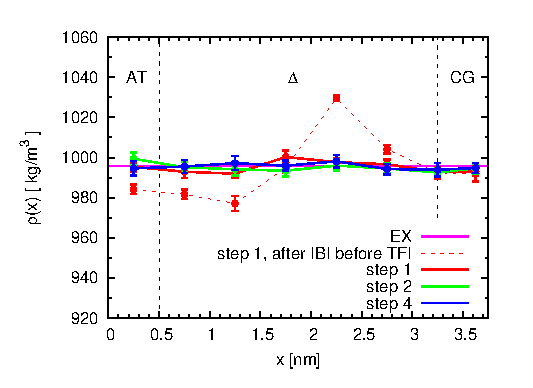
\includegraphics{fig.3/rho.eps}
  \caption{The resulting $\rho(x)$ of the IBI-TFI correction loop.
    The results of the first iteration is colored by red. Within the
    first iteration, the density profile after the IBI and before the
    TFI is denoted by the  red dashed line.  After the TFI, the density
    profile is denoted by the  red solid line.  The second and third
    steps are denoted by green and blue solid lines,
    respectively. Both of them are the density profiles after the
    whole IBI-TFI iteration. The ideal uniform density profile is
    denoted by the solid pink line for reference. The bar on the data
    points denotes the statistical uncertainty (with a confidence
    interval of 95\%). EX, HY and CG are denoting the atomistic
    (explicit), hybrid and coarse-graining regions, respectively. }
  \label{fig:tmp3}
\end{figure}

\begin{figure}
  \centering
  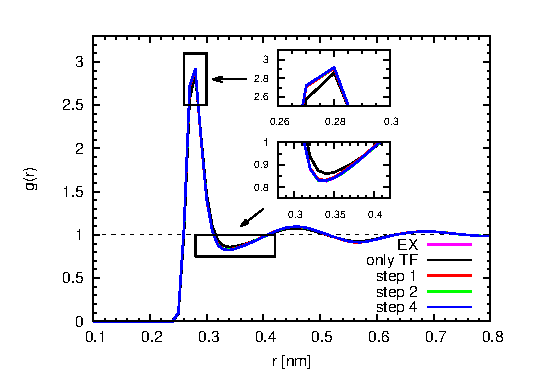
\includegraphics{fig.3/rdf.eps}
  \caption{The resulting $g(r)$ of the IBI-TFI correction loop.  The
    RDF of after the first, second and the third step iteration are
    denoted by red, green and blue solid lines, respectively.  The
    atomistic RDF is presented by pink solid line, which is
    overlapping with the other lines, and cannot be seen from the
    plot. The RDF with thermodynamic force correction but without RDF
    correction is presented by black line for reference. Two subplots
    are inserted in the figure to show zoom-in of the RDFs at the
    first peak and the first valley.}
  \label{fig:tmp4}
\end{figure}


\subsection{Numerical results}

The testing system contained 3456 SPC/E \cite{berendsen1987missing}
water molecules in a $7.50\textsf{nm}\times 3.72\textsf{nm}\times
3.72\textsf{nm}$ periodic box. The system was split in $x$ direction
into one explicit region of width $1.00\textsf{nm}$ and one
coarse-grained region of width $1.00\textsf{nm}$ connected by two
hybrid region of width $2.75\textsf{nm}$. The simulation was made at
room temperature of $300\textsf{K}$. The time step was $\Delta t =
0.002\textsf{ps}$. The cut-off radius used for all interactions was
$0.90\textsf{nm}$. The electrostatic interaction method used for the
explicit region was the reaction field method. All simulations were
performed by MD simulation software Groamcs \redc{citations please!}
and VOTCA \cite{ruehle2009versatile}.

Using the IBI-TFI correction loop,
the convergence of the density $\rho(x)$ and RDF $g(r)$ are presented
in Fig.~\ref{fig:tmp3} and \ref{fig:tmp4}, respectively. After the
first step of the IBI-TFI iteration, the density profile obviously
deviates from the perfect uniform density distribution, but it
converges to uniform distribution after the third step of the
iteration. In Fig. \ref{fig:tmp4}, we also show the RDF of AdResS
simulation without RDF correction (with thermodynamic force applied),
and a clear discrepancy with the atomistic RDF is presented,
that is why the RDF correction is necessary.  By
the IBI-TFI iteration, the RDF converges to the atomistic RDF very
fast. Therefore, the proposed IBI-TFI loop (Algorithm \ref{algo:1}) is
a robust and fast converging method.

\begin{figure}
  \centering
  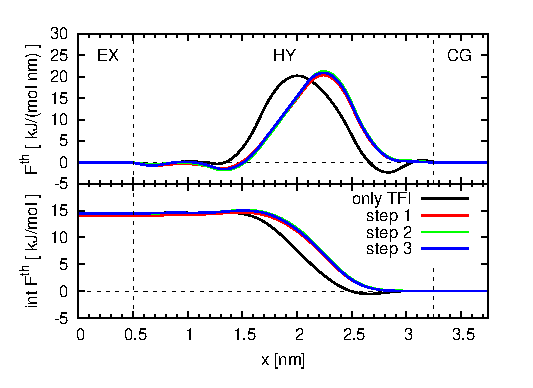
\includegraphics{fig.2/tf-and-int.eps}
  \caption{The resulting $\v F^{\textrm{tf}}$ of the IBI-TFI
    correction loop.  The thermodynamic force $\v F^{\textrm{tf}}$ (in
    this case, only the $x$ component is non-zero) and its integration
    (from positive to negative) after the first, second and the third
    step iteration are denoted by red, green and blue solid lines,
    respectively.  The thermodynamic force without RDF correction,
    which is used as initial guess for the TFI-IBI loop, is plotted
    for comparison. EX, HY and CG are denoting the atomistic
    (explicit), hybrid and coarse-graining regions, respectively.}
  \label{fig:tmp5}
\end{figure}

\begin{figure}
  \centering
  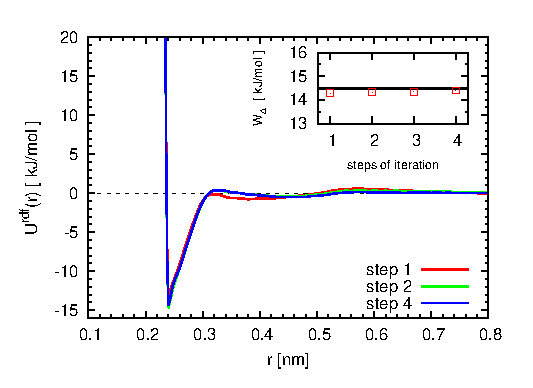
\includegraphics{fig.3/force-rdf.eps}
  \caption{The resulting $U^{\textrm{rdf}}(r)$ of the IBI-TFI
    correction loop.  The $U^{\textrm{rdf}}(r)$ after the first,
    second, third and fourth step iteration are denoted by red, green,
    blue and cyan solid lines, respectively.  }
  \label{fig:tmp6}
\end{figure}

In the upper plot of Fig. \ref{fig:tmp5} presents the thermodynamic
force, and the lower plot is the integration of
the thermodynamic force from positive to negative direction, which
presents the grand potential (i.e. $-pV$) difference with the
coarse-grained representation~\cite{fritsch2011grand}.
The thermodynamic force converges very
fast, we cannot see obvious difference between the second
step and the third step.  In Fig. \ref{fig:tmp5} we also show the
thermodynamic force without RDF correction for comparison. The force
without RDF correction is different from those with RDF
correction. Noticing at around $x=2.7 \textsf{nm}$, the force is
negative, and the integrated force forms a shallow attractive well,
which corresponding to an unphysical tendency of aggregation of molecules. The RDF
correction fixes this problem. From the lower plot of
Fig. \ref{fig:tmp5}, the grand potential difference between the
atomistic region and the coarse-grained region is preserved by the
IBI-TFI loop, which means that the equivalence of the chemical
potential (?) achieved by the thermodynamic
force~\cite{fritsch2011grand} is preserved by the RDF correction.

Fig. \ref{fig:tmp6} presents the convergence of the RDF correction
potential (negative gradient is the force). The potential is almost 0
when $r > 3.1\textsf{nm}$. This means that the RDF correction is
basically targeting at the first neighbor shell. After step 3, the RDF
correction force converges very good at $r > 2.6\textsf{nm}$. Two
particles have only little possibility to get closer than $2.6\textsf{nm}$,
see the RDF in Fig. \ref{fig:tmp4}, so the bad convergence at $r <
2.6\textsf{nm}$ is not a big problem, that is also the reason why the
RDF converges very good after only two steps of iterations.

% \begin{figure}
%   \centering
%   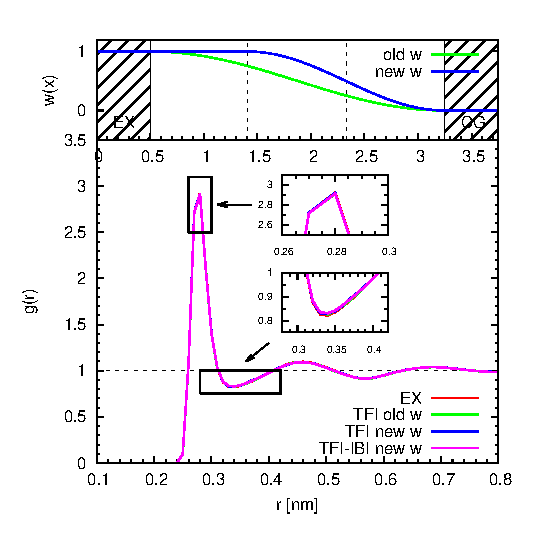
\includegraphics[width=0.49\textwidth]{fig/rdf-ex-cg.eps}
%   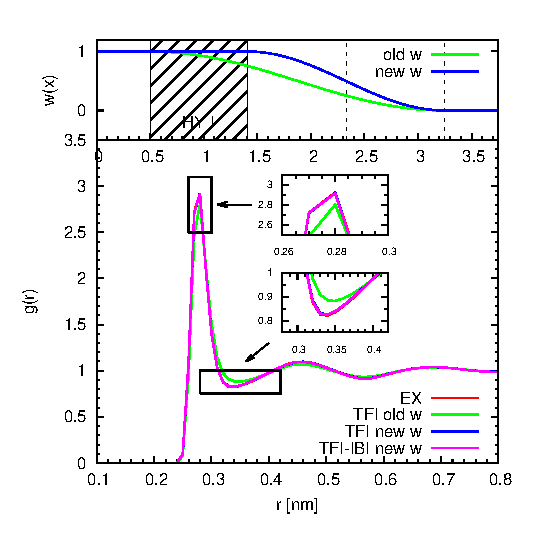
\includegraphics[width=0.49\textwidth]{fig/rdf-425-516.eps}
%   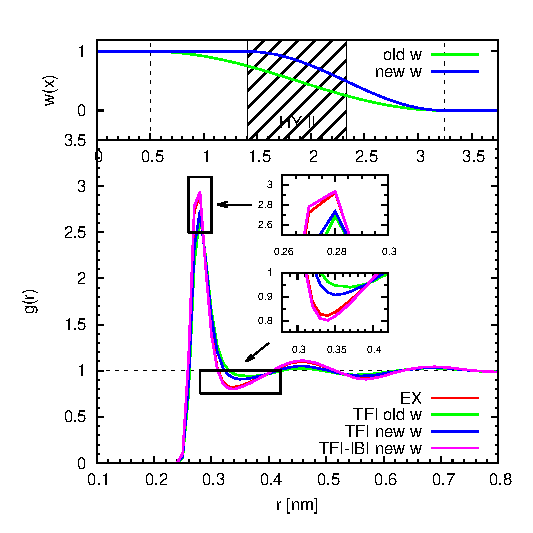
\includegraphics[width=0.49\textwidth]{fig/rdf-516-608.eps}
%   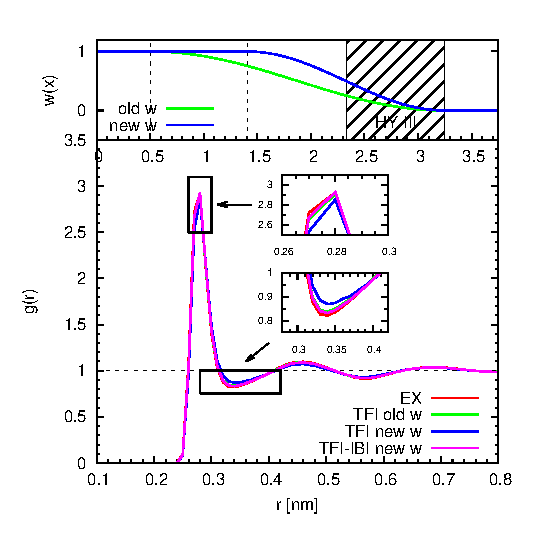
\includegraphics[width=0.49\textwidth]{fig/rdf-608-700.eps}
%   \caption{The regional RDFs. The red line is the RDF of the atomistic
%     simulation. The thermodynamic force simulation without RDF
%     correction using the old weighting function \eqref{eqn:old-w} and
%     the new weighting function \eqref{eqn:new-w} are denoted by the
%     green and blue line, respectively. The RDF of the proposed TFI-IBI
%     method is denoted by the pink line. The hybrid region is equally
%     divided into three parts: HY I, HY II and HY III, the width of
%     which are rough the cut-off radius, i.e. 9 \textsf{nm}. Two
%     subplots are inserted in the plot to show zoom-in of of RDFs at
%     the first peak and the first valley.  }
%   \label{fig:tmp7}
% \end{figure}


\begin{figure}
  \centering
  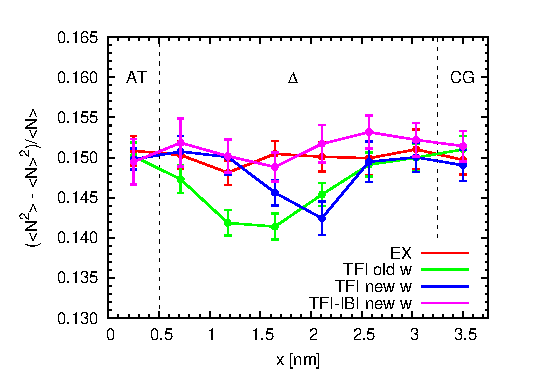
\includegraphics[]{fig.3/count.eps}
  \caption{
    The molecular number fluctuation.
    The red line is the fluctuation of the atomistic
    simulation. The thermodynamic force simulation without RDF
    correction using the old weighting function \eqref{eqn:old-w} and
    the new weighting function \eqref{eqn:new-w} are denoted by the
    green and blue line, respectively. The fluctuation of the proposed TFI-IBI
    method is denoted by the pink line.  }
\end{figure}


\begin{figure}
  \centering
  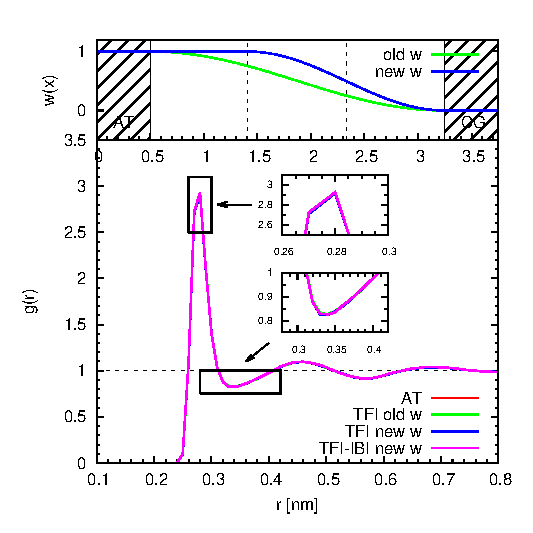
\includegraphics[width=0.49\textwidth]{fig.3/rdf-ex-cg.eps}
  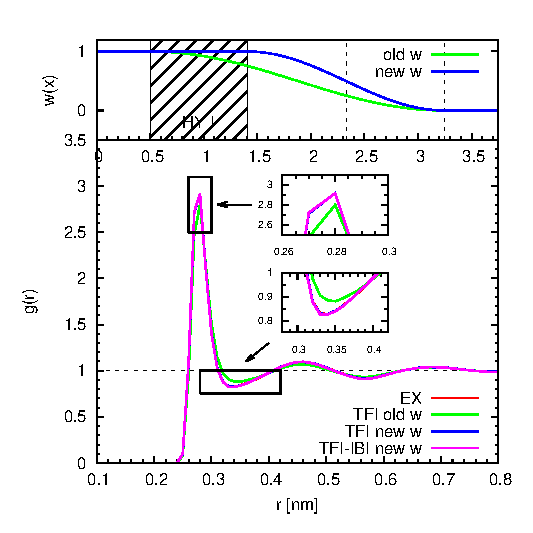
\includegraphics[width=0.49\textwidth]{fig.3/rdf-425-516.eps}
  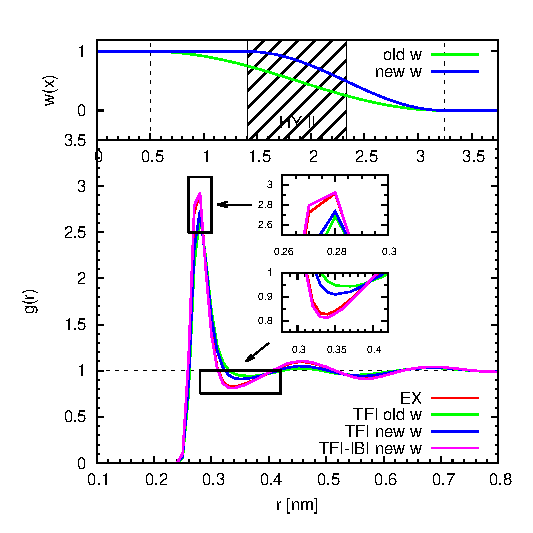
\includegraphics[width=0.49\textwidth]{fig.3/rdf-516-608.eps}
  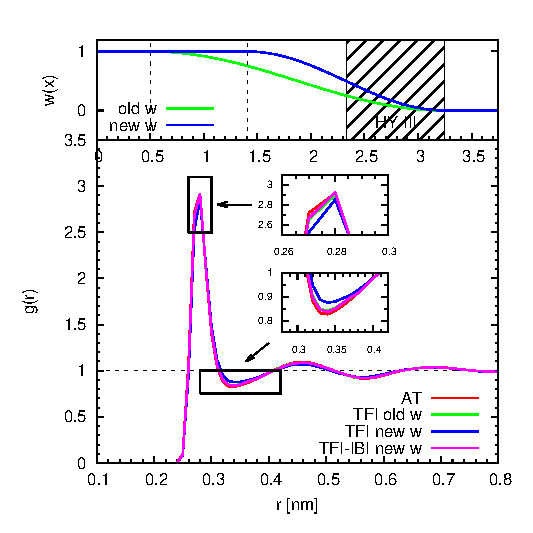
\includegraphics[width=0.49\textwidth]{fig.3/rdf-608-700.eps}
  \caption{The regional RDFs. The red line is the RDF of the atomistic
    simulation. The thermodynamic force simulation without RDF
    correction using the old weighting function \eqref{eqn:old-w} and
    the new weighting function \eqref{eqn:new-w} are denoted by the
    green and blue line, respectively. The RDF of the proposed TFI-IBI
    method is denoted by the pink line. The hybrid region is equally
    divided into three parts: HY I, HY II and HY III, the width of
    which are rough the cut-off radius, i.e. 9 \textsf{nm}. Two
    subplots are inserted in the plot to show zoom-in of of RDFs at
    the first peak and the first valley.  }
  \label{fig:tmp7}
\end{figure}


We plot the regional RDF in Fig. \ref{fig:tmp7}. Three methods are
compared: the AdResS with the old \eqref{eqn:old-w} and the new
weighting function, and the proposed TIF-IBI correction loop
method. In the explicit and coarse-grained region, the RDF all method
are consistent with the explicit simulation. The hybrid region is
divided into three parts: HY I, HY II and HY III, the width of which
are roughly the cut-off radius. In region HY I, the new weighting
function is 1, so the methods using new weighting function give
correct RDF. In region III, the TFI with new weighting function is not
correct, but surprisingly, the TFI with old weighting function gives
better result. In both the regions, the RDF of TFI-IBI is consistent
with the atomistic simulation, which is one of the necessary condition
to produce correct grand-canonical sampling.  In region HY II, the
methods without RDF correction deviate far from the atomistic
simulation. The TFI-IBI method is also not perfect, however, the worse
results in HY II do not seriously disturb the results in HY I and HY
III. Fig. \ref{fig:tmp7} presents why the RDF correction is important
to satisfy the necessary conditions for grand-canonical simulation.


\section{Conclusions}
\label{sec:conclusions}

% \redc{STILL MISSING: simulation protocol. do not forget citing Gromacs and VOTCA}

% \newpage

\bibliography{ref}{}
\bibliographystyle{unsrt}

\end{document}
